% !TEX root = ../../document.tex

\documentclass{subfiles}

\begin{document}

  \chapter{Métodos de Resolución}
  \label{chap:solving}

    \section{Introducción}
    \label{sec:solving_introduction}

      \paragraph{}
      Los problemas de \emph{optimización combinatoria} constituyen una de las categorías más interesantes dentro del área de la optimización de variables. Esto se debe a la gran aplicabilidad de los mismos en situaciones de la vida real, así como la gran reducción de costes que se puede alcanzar cuando estos son aplicados en los puntos estratégicos de cualquier proceso de producción.

      \paragraph{}
      Sin embargo, esta categoría de problemas de optimización presenta un mayor grado de dificultad en su resolución, tal y como se ha indicado a lo largo del \cref{chap:formulation}. Entre otros, esto se debe a la imposibilidad de utilizar técnicas basadas en gradientes (que en problemas con variables de decisión continuas proporcionan simplifican mucho su resolución). Puesto que estas técnicas no son aplicables, la estrategia alternativa se basa en la enumeración de posibles configuraciones de variables de manera inteligente hasta alcanzar aquella que genere el resultado óptimo para la instancia del problema que se pretenda resolver.

      \paragraph{}
      Por tanto, a pesar de no ser posible el apoyo en técnicas basadas en gradientes, si que existe la aternativa basada en enumeración de configuraciones como enfoque para dar con el óptimo. A pesar de ello, es fácil darse cuenta de que esta estrategia no es lo suficientemente potente como para permitir resolver problemas reales (o incluso de pequeño tamaño). La dificultad radica en la explosión combinatoria generada por la enumeración de soluciones. Por ejemplo, en un problema compuesto por $20$ variables de decisión de naturaleza binaria, el número de configuraciones a evaluar alcanzaría el valor de $2^{20} = 1048576$, lo cual no es escalable a problemas de gran tamaño, donde hay cientos o miles de variables de decisión con las que trabajar.

      \paragraph{}
      A pesar de esta dificultad, es posible enfrentarse a problemas de \emph{optimización combinatoria} de tamaños relativamente grande teniendo en cuenta distintas estrategias que permiten ignorar un gran número de configuraciones no factibles dadas las restricciones descritas por el problema en cuestión. Es por ello que muchos de los métodos de resolución se apoyan en estas garantias para enfocar la búsqueda sobre un subespacio de configuraciones factibles. Otra de las ideas más utilizadas por los métodos de resolución es apoyarse en los resultados de evaluación de configuraciones anteriores para que el coste computacional de evaluación de configuraciones actuales sea mucho menor. Dicha estrategia algorítmica se conoce como \emph{Programación Dinámica}, la cual se describe en mayor detalle en \cite{bellman1954theory}.


      \paragraph{}
      A lo largo del capítulo se decriben distintas situaciones en que es posible aplicar las técnicas anteriormente descritas sobre el \emph{problema Dial-a-Ride} para tratar de reducir en la medida de los posible la complejidad computacional que este presenta. Entonces, el resto del capítulo se organiza de la siguiente manera: En el \cref{sec:solving_exacts} se describen las distintas técnicas de resolución exactas que la literatura especializada en el problema a probado para tratar de resolver el problema. Seguidamente, en el \cref{sec:solving_heuristics} se describen estrategia basadas en heurísticas (tanto de construcción como mejora de soluciones) que a pesar de no ofrecer ninguna garantía de optimalidad, ofrecen un buen equilibrio entre tiempo de cómputo y calidad de las soluciones. Después, en el \cref{sec:solving_metaheuristics} se describen un conjunto de metaheurísticas basadas en la utilización de las heurísticas descritas en el apartado anterior de manera inteligente de tal manera que las configuraciones generadas proporcionan soluciones de mayor calidad. Por último, en el \cref{sec:solving_conclusions} se incluyen unas conclusiones generales acerca de los métodos de resolución aplicados al \emph{problema Dial-a-Ride}.

    \section{Métodos de Resolución Exactos}
    \label{sec:solving_exacts}

      \paragraph{}
      Los métodos de resolución exactos representan una de las categorías de resolución de problemas de optimización más interesantes debido a distintos factores, entre los que se encuentran aquellas situaciones en que es estrictamente necesario obtener el valor óptimo para una instancia dada. Sin embargo, esta categoría no solo es interesante por dicha razón, sino que el estudio de estos problemas además proporciona en muchas ocasiones razonamientos y justificaciones teóricas sobre el problema que pretenden resolver que ayudan a comprender mejor los factores del mismo. Lo interesante de este punto es que esto sirve de utilidad para el diseño de diferentes métodos de resolución así como su justificación.

      \paragraph{}
      Tal y como se ha descrito anteriormente, el método de resolución exacta más básico consiste en la enumeración de todas las configuraciones posibles dadas la variables de decisión del problema para después determinar como configuración óptima aquella que maximiza/minimiza la función objetivo. Esto es teóricamente posible por la naturaleza combinatoria del problema pero a la vez prácticamente imposible por la misma razón.

      \paragraph{}
      Puesto que los problemas de \emph{optimización combinatoria} se pueden modelar como problemas de \emph{optimización lineal} mediante un conjunto de restricciones de naturaleza lineal, la siguiente alternativa a la enumeración de configuraciones es la resolución como un problema de esta naturaleza. Para ello, una de las opciones es la utilización del algoritmos \emph{Simplex} \cite{klee1970good} tal y como se indica en el \cref{sec:formulation_linear_problems}. Como se ha descrito anteriormente, este algoritmo se basa en la búsqueda de la mejor solución contigua a la actual de manera iterativa hasta alcanzar aquella que no tenga una solución contigua mejor. Es posible demostrar que este algoritmo  alcanza el valor óptimo cuando se aplica sobre problema de \emph{optimización lineal}. Tal y como se puede apreciar en la \cref{img:solving_simplex}, gráficamente puede ser visto como la evaluación de vértices en un grafo de soluciones. La complejidad que esta estrategia presenta en problemas de \emph{optimización combinatoria} reside en el gran número de vértices que surgen del cambio de valor de cada una de las variables de decisión del problema, generando un grafo con gran número de vértices y aristas lo cual hace inalcanzable computacionalmente navegar por el mismo hasta alcanzar la solución óptima.

      \begin{figure}[ht]
        \centering
        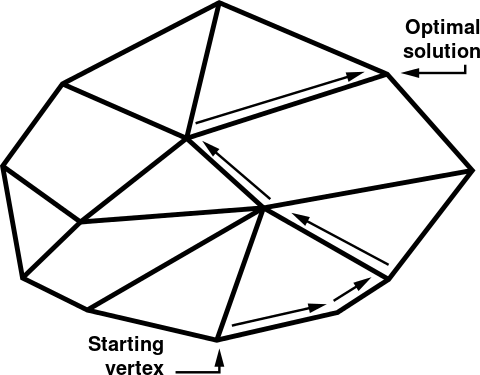
\includegraphics[width=0.4\textwidth]{simplex-graphically}
        \caption{Representación gráfica del modo de ejecución del algoritmo \emph{Simplex}.}
        \label{img:solving_simplex}
      \end{figure}

      \subsection{Branch and Bound}
      \label{sec:solving_branch_bound}

        \paragraph{}
        [TODO]

      \subsection{Branch and Cut}
      \label{sec:solving_branch_cut}

        \paragraph{}
        [TODO]

      \subsection{Branch and Price}
      \label{sec:solving_branch_price}

        \paragraph{}
        [TODO]

      \subsection{Branch and Cut and Price}
      \label{sec:solving_branch_cut_price}

        \paragraph{}
        [TODO]

      \paragraph{}
      [TODO]

    \section{Métodos de Resolución basados en Heurísticas}
    \label{sec:solving_heuristics}

      \paragraph{}
      [TODO]

      \subsection{Greedy}
      \label{sec:solving_greedy}

        \paragraph{}
        [TODO]


        \paragraph{}
        \begin{algorithm}
          \SetAlgoLined
          \KwResult{$E'$ }
          $S \gets \emptyset$\;
          \While{$A \neq \emptyset$}{
            $o \gets \text{best(A)}$\;
            $S \gets S \cup \{ o \}$\;
            $A \gets A \cap \{ o \}$\;
          }
          \caption{[TODO]}
          \label{code:solving_greedy}
        \end{algorithm}


        \paragraph{}
        [TODO]

        \subsubsection{Criterios de Selección}
        \label{sec:solving_greedy_criterions}

          \paragraph{}
          [TODO]

        \subsubsection{Randomized Greedy}
        \label{sec:solving_randomized_greedy}

          \paragraph{}
          [TODO]

      \subsection{Metropolis Hastings}
      \label{sec:solving_metropolis}

        \paragraph{}
        [TODO]

      \paragraph{}
      [TODO]

    \section{Métodos de Resolución basados en Metaheurísticas}
    \label{sec:solving_metaheuristics}

      \paragraph{}
      [TODO]

      \subsection{GRASP}
      \label{sec:solving_grasp}

        \paragraph{}
        [TODO]

      \subsection{Simulated Anneling}
      \label{sec:solving_simulated_anneling}

        \paragraph{}
        [TODO]

      \subsection{Tabu Search}
      \label{sec:solving_tabu}

        \paragraph{}
        [TODO]

      \subsection{Ant Colony}
      \label{sec:solving_ant_colony}

        \paragraph{}
        [TODO]

      \subsection{Variable Neighborhood Search}
      \label{sec:solving_vns}

        \paragraph{}
        [TODO]

      \subsection{Large Neighborhood Search}
      \label{sec:solving_lns}

        \paragraph{}
        [TODO]

      \paragraph{}
      [TODO]

    \section{Conclusiones}
    \label{sec:solving_conclusions}

      \paragraph{}
      [TODO]

\end{document}
